% Generated by pptx_to_beamer.py
\documentclass{beamer}
\usetheme{Madrid}
\usepackage{graphicx}
\usepackage{hyperref}
\usepackage{amsmath}
\usepackage{booktabs}
\usepackage[utf8]{inputenc}
\usepackage{textgreek}

\title{Line Methods and Direction Set Methods in Multidimensional Optimization}
\date{\today}

\begin{document}

\begin{frame}
  \titlepage
\end{frame}

\begin{frame}{From 10.6 (linmin) to 10.7 (Powell’s Method)}
\end{frame}

\begin{frame}{What Does It Mean to Minimize a Function?}
\begin{itemize}
  \item Goal:
  \item A function that maps inputs to outputs
  \item We want the input that produces the smallest output
  \item Example: f(x) = (x - 3)\textasciicircum{}2, minimum occurs at x = 3, f(3) = 0
\end{itemize}
  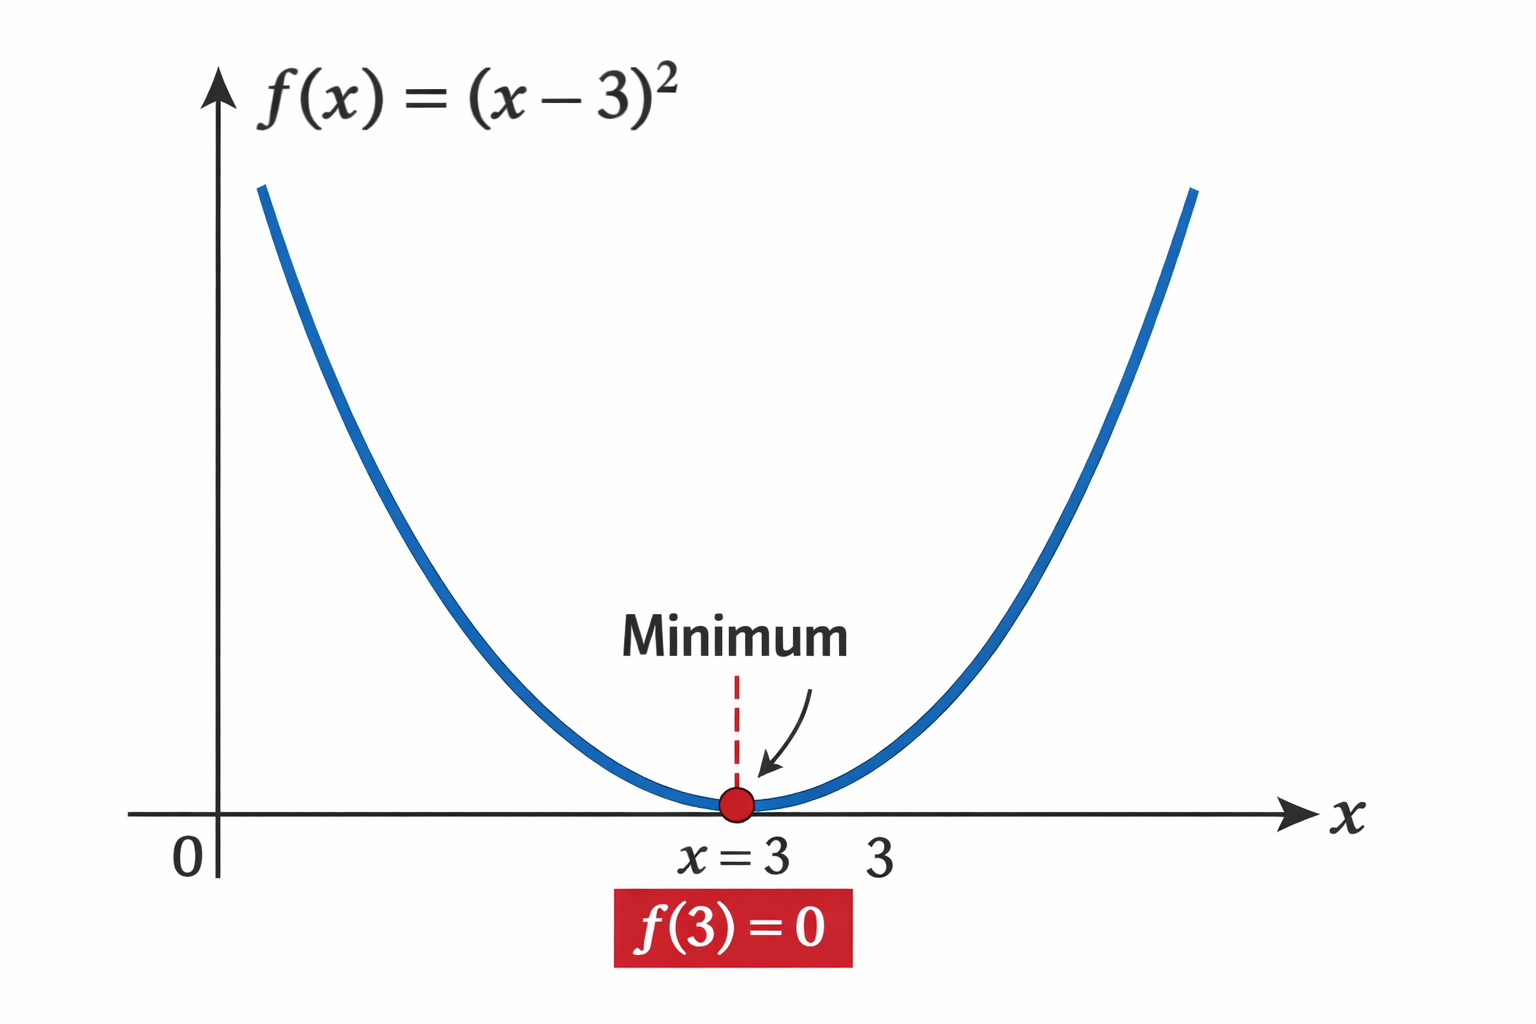
\includegraphics[width=0.8\textwidth]{beamer_images/slide2_img1.png}
\end{frame}

\begin{frame}{From One Variable to Many Variables}
\begin{itemize}
  \item One variable: f(x)
  \item Many variable: f(x,y), f(x,y,z), f(x)
  \item Represents a surface or landscape
  \item Hard to search directly
  \item Analogy: Finding the lowest point on a mountain
\end{itemize}
  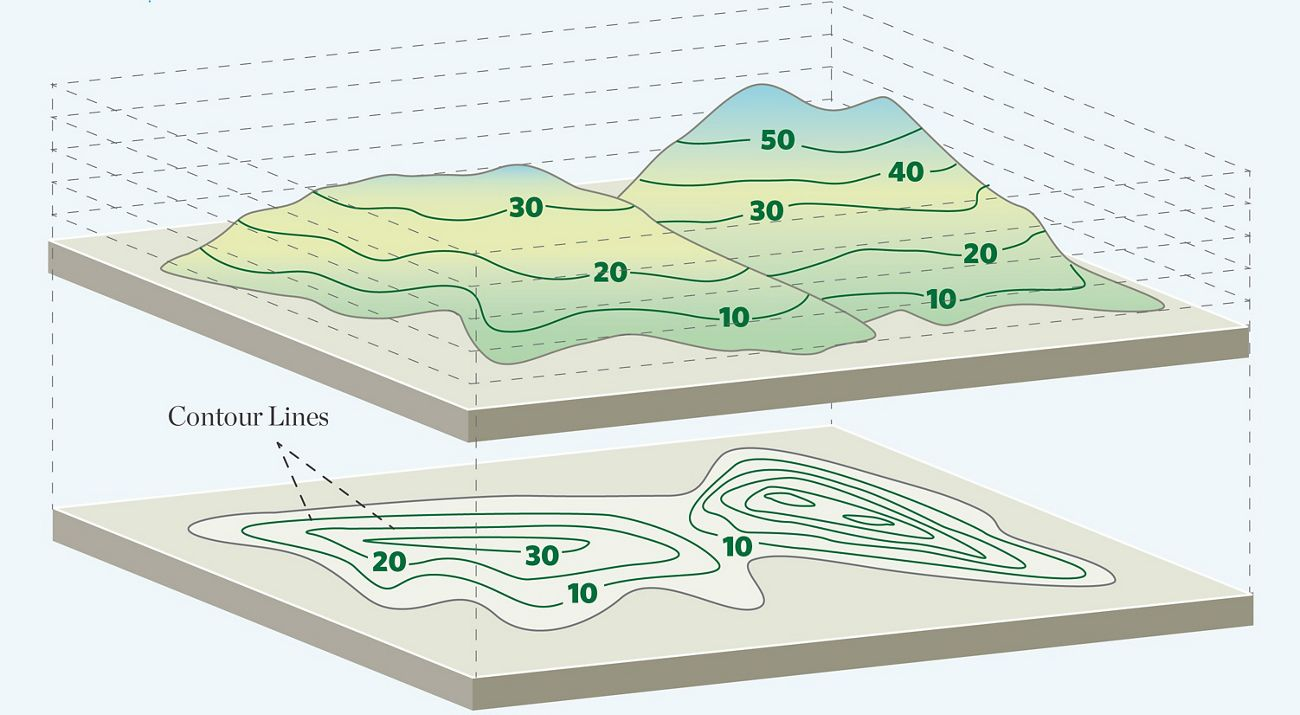
\includegraphics[width=0.8\textwidth]{beamer_images/slide3_img1.png}
\end{frame}

\begin{frame}{Key Idea of 10.6: Reduce to One Dimension}
\begin{itemize}
  \item Instead of searching everywhere:
  \item Pick a starting point
  \item Pick a direction
  \item Move along that straight line
  \item Mathematically:
  \item x(t)=p+tξ
  \item Define :
  \item g(t)=f(p+tξ)
  \item Thus the problem is now a one dimensional problem
\end{itemize}
  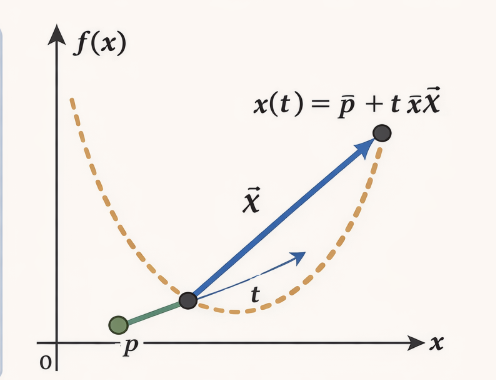
\includegraphics[width=0.8\textwidth]{beamer_images/slide4_img1.png}
\end{frame}

\begin{frame}{What linmin Does (10.6)}
\begin{itemize}
  \item Input:
  \item Current point, p
  \item Direction, ξ
  \item function , f
  \item Output:
  \item Moves p to the min along that line
  \item Returns the function value
\end{itemize}
  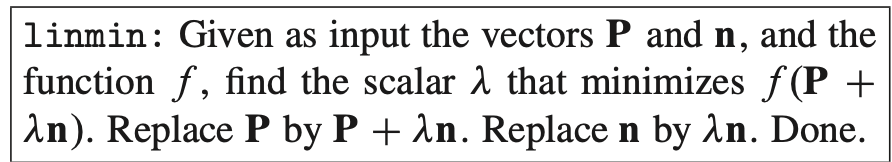
\includegraphics[width=0.8\textwidth]{beamer_images/slide5_img1.png}
\end{frame}

\begin{frame}{Big Question: Which direction should we choose next}
\begin{itemize}
  \item From 10.6 we already know how to move to the best point along one chosen direction using linmin()
  \item If we choose directions poorly, the algorithm can be extremely slow.
\end{itemize}
  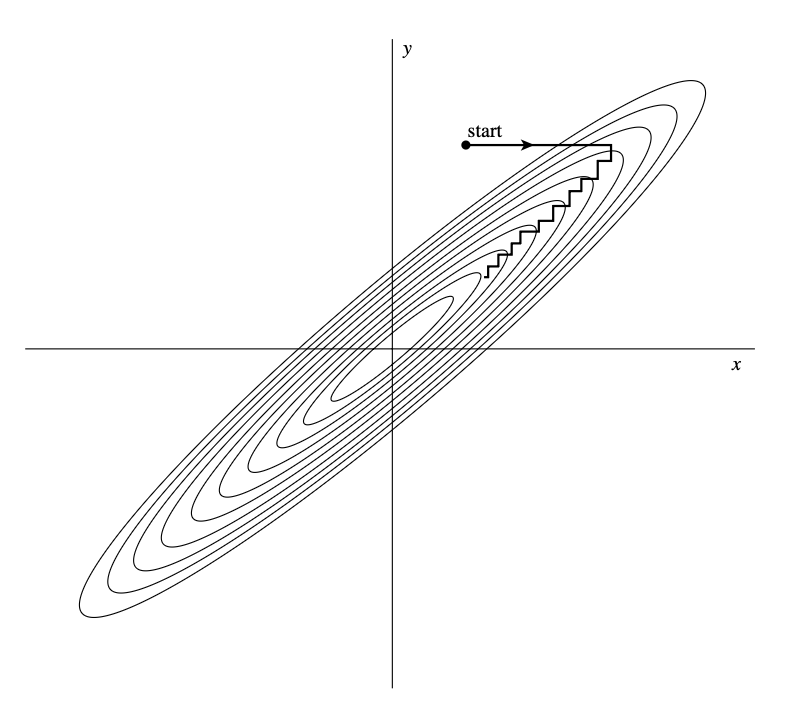
\includegraphics[width=0.8\textwidth]{beamer_images/slide6_img1.png}
\end{frame}

\begin{frame}{Goal of Direction Set Methods (10.7)}
\begin{itemize}
  \item Instead of fixed directions:
  \item Update directions as the algorithm runs.
  \item Learn directions that follow valleys.
  \item Avoid undoing previous progress.
  \item Goal:
  \item Move efficiently toward the minimum.
\end{itemize}
\end{frame}

\begin{frame}{Conjugate Directions}
\begin{itemize}
  \item Two directions are \textbf{conjugate} if:
  \item Moving along one does not ruin the minimization along the other.
  \item If we find N conjugate directions:
  \item A quadratic function can be minimized in N line searches.
  \item Key idea:
  \item Directions should not interfere with each other.
\end{itemize}
\end{frame}

\begin{frame}{Powell’s Method}
\begin{itemize}
  \item Start with coordinate directions.
  \item Run linmin along each direction.
  \item Measure the net movement direction.
  \item Add this new direction.
  \item Remove one old direction.
  \item Repeat until improvement is small.
\end{itemize}
  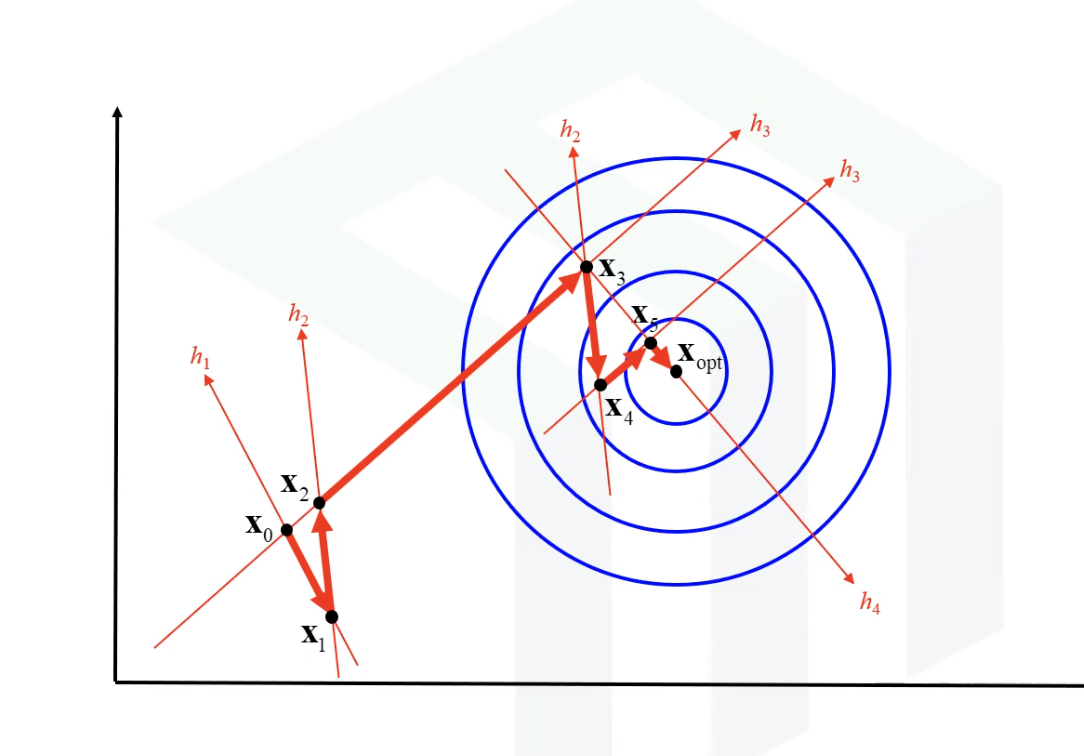
\includegraphics[width=0.8\textwidth]{beamer_images/slide9_img1.png}
\end{frame}

\begin{frame}{Overall Summary}
\begin{itemize}
  \item Why powell works better:
  \item Learns good directions automatically
  \item Avoids zig-zagging
  \item Faster convergence than coordinate descent
  \item Works without gradients
\end{itemize}

\begin{block}{}
10.6: How to move optimally along one direction (linmin).
10.7: How to choose and update directions intelligently (Powell).
Together they solve multidimensional minimization efficiently.
\end{block}
\end{frame}

\end{document}
